\newpage
\section{Durchführung}
    \subsection{Versuchsaufbau}

        \FloatBarrier

        \begin{figure}[h]
          \centering
          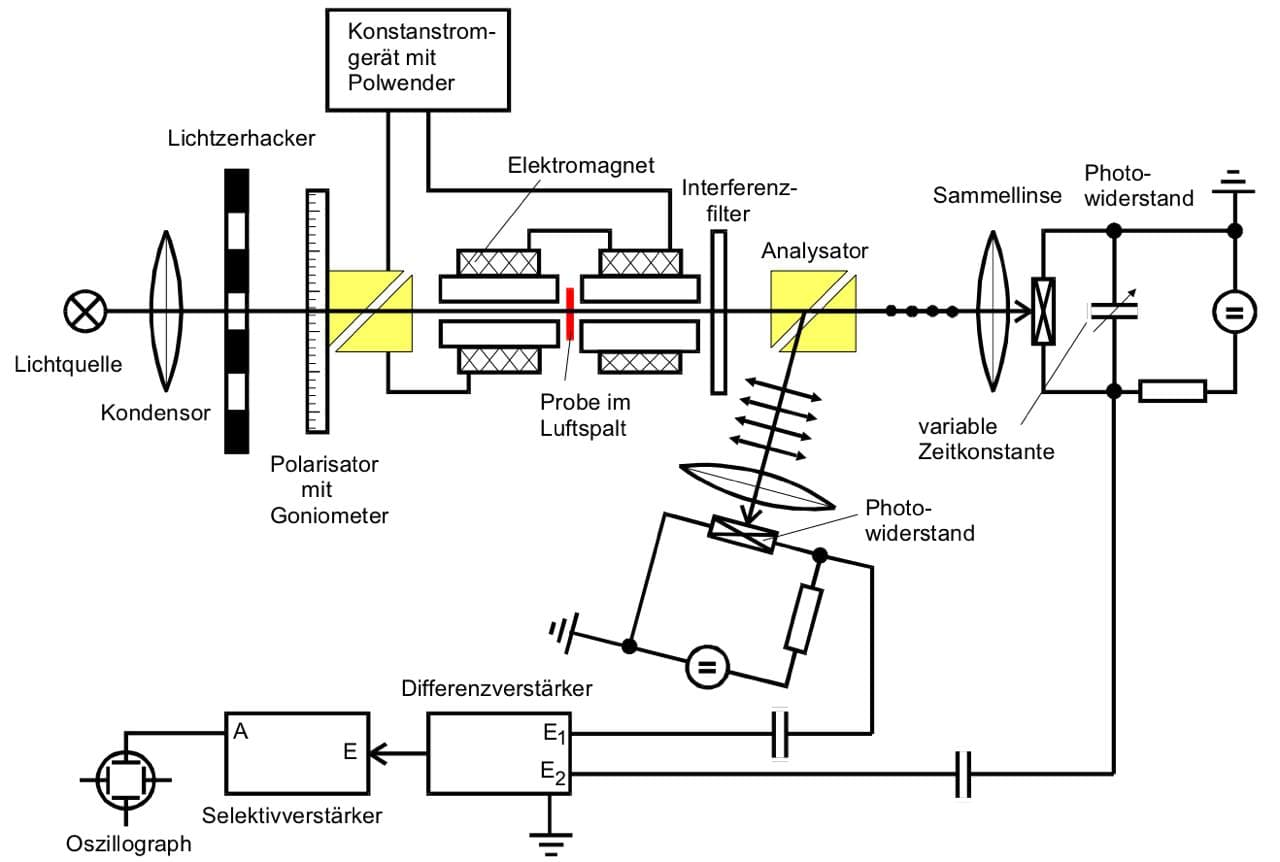
\includegraphics[width = 0.9\textwidth]{pictures/Aufbau.jpg}
          \caption{In der Abbildung ist der Aufbau zur Messung des Faraday-Rotationswinkels dargestellt. Zum Auftreten des Effekts sind die Elektromagneten essenziell, in deren magnetischen Feld das linear polarisierte Licht aus der Halogen-Lampe die Halbleiter-Probe durchläuft. Nach Verlasssen des Elektromagnetenaufbaus wird der Strahl im Analaysator in zwei senkrecht zueinander polarisierte Strahlen  aufgeteilt und auf Photowiderstände fokussiert. Selektiv- und Differenzverstärker geben ein Signal auf dem Oszilloskop aus, wenn die beiden Teilstrahlen die ungleiche Intensitäten haben. Entnommen aus~\cite{tu_dortmund_versuchsanleitung_2021-2}}
          \label{fig:Aufbau}
        \end{figure}

        \FloatBarrier

        \noindent
        Der Ausgangspunkt des in Abbildung~\ref{fig:Aufbau} zu sehenden experimentellen Aufbaus ist eine Halogen-Lampe, die vorwiegend Licht im infraroten Bereich aussendet. Dieses wird kollimiert und trifft auf einen Polarisator, der den Polarisationswinkel des Lichts einstellen und per Goniometer ablesen lässt. Im Strahlengang befindet sich ein sogenannter Zerhacker, der einer Scheibe mit einer Öffnung entspricht, die mit einer vorgegebenen Frequenz rotiert, sodass der Lichtstrahl mit dieser Frequenz gepulst wird. Um die Faraday-Rotation zu messen, durchquert der Strahl einen durchbohrten Elektromagneten, dessen Magnetfeld durch Umpolung parallel oder anti-parallel zur Ausbreitungsrichtung des Strahls ausgerichtet werden kann. Innerhalb des Elektromagnetenaufbaus ist eine Halterung, in die eine Probe des Materials, dessen effektive Elektronenmasse gemessen werden soll, platziert werden kann. Nach Durchlaufen dieses Mediums und Verlassen des Elektromagnetenaufbaus, trifft der Strahl auf einen Interferenzfilter, der den Strahl monochromatisiert. Diese Interferenzfilter werden variiert, sodass die Faraday-Rotation für verschiedene Wellenlängen gemessen werden kann. Nach der Monochromatisierung wird der Strahl durch ein weiteres Glan-Thompson-Prisma in zwei Teilstrahlen zerlegt, die senkrecht zueinander polarisiert sind. Beide Strahlen werden auf jeweils einen Photowiderstand fokussiert, deren Messspannungen auf einen Differenzverstärker geleitet werden. Dieser gibt ein Signal aus, das proportional zu der Differenz der beiden Strahlenintensitäten ist. Auf den Differenzverstärker folgt ein Selektivverstärker, der Signale einer ausgewählten Frequenz verstärkt und auf ein Oszilloskop ausgibt. In diesem Fall entspricht die Frequenz der des Zerhackers, um andersweitiges Rauschen, wie das der künstlichen Beleuchtung zu unterdrücken und nur das Licht der Halogen-Lampe zu detektieren.

    \subsection{Justierung}
        Bevor die Messung durchgeführt werden kann, muss der Aufbau justiert werden. Zunächst wird überprüft, ob das Glan-Thompson-Prisma korrekt funktioniert, indem der Polarisator und das Prisma so 
        zueinander ausgerichtet werden, dass kein Licht durch das Prisma transmittiert wird. Dies kann visuell überprüft werden. \newline
        Anschließend werden die Linsen und dahinter befindlichen Photowiderstände so ausgerichtet, dass die beiden aus dem zweiten Glan-Thompson-Prisma austretenden Teilstrahlen jeweils auf die Photowiderstände
        fokussiert werden. Auch dies kann visuell über den sichtbaren Anteil des Lichts verifiziert werden, sofern kein Interferenzfilter den sichtbaren Teil des Strahls ausfiltert. \newline
        Um das Signal der auf die Photowiderstände treffenden Teilstrahlen vor möglichem Hintergrundrauschen abzuheben, wird die Frequenz des Selektivverstärkers zunächst auf die Frequenz des Zerhackers eingestellt und anschließend so feinjustiert, dass das vom Oszilloskop angezeigte Ausgangssignal maximiert wird.  
    \subsection{Messungen}
        \subsubsection*{Bestimmung der magnetischen Flussdichte}
            Da der Rotationswinkel des Faraday-Effekts proportional zur magnetischen Flussdichte B ist, muss diese am Ort der Probe bestimmt werden. Dazu wird eine Hall-Sonde durch die Bohrung in den Elektromagneten eingeführt und so die magnetische Flussdichte in Abhängigkeit zum relativen Abstand zur Probenposition gemessen. Diese Messung wird für beide Polarisierungen des Elektromagneten durchgeführt und die Beträge der Flussdichten verglichen.
        \newpage   
        \subsubsection*{Messung der Faraday-Rotation}
            Zur Bestimmung der effektiven Elektronenmasse müssen die Faraday-Rotationen gemessen werden. Dazu wird die maximale magnetische Flussdichte $\text{B}_{\text{max}}$ angelegt und der Polarisator auf einen Winkel $\theta_1$ eingestellt, bei dem die Differenzspannung verschwindet. Daraufhin wird das Feld umgepolt und der Polarisator vom zuvorigen Winkel zum nächsten Winkel $\theta_2$ gedreht, an dem die Differenzspannung erneut verschwindet. Da das Umpolen des Feldes einer Änderung der magnetischen Flussdichte um $2\text{B}_{\text{max}}$ entspricht, lässt sich der Rotationswinkel zu 
            \begin{equation}
                \theta = \frac{\theta_1 - \theta_2}{2}
                \label{eqn:zweiwinkel}
            \end{equation}
            bestimmen. Dieses Vorgehen wird für folgende Proben der Länge L und der Donatorenkonzentration N
            \begin{enumerate}
                \item GaAs (n-dotiert), L=\SI{1.360}{\milli\metre}, N=\SI{1.2e18}{\per\cubic\centi\metre}
                \item GaAs (n-dotiert), L=\SI{1.296}{\milli\metre}, N=\SI{2.8e18}{\per\cubic\centi\metre}
                \item GaAs (hochrein), L=\SI{5.110}{\milli\metre}
            \end{enumerate}
            

            und jeweils neun verschiedene Interferenzfilter wiederholt.

        
